\section{Theory ATED}

\subsection{Refinement Awareness}
\label{sec:refinement-awareness}

One of the biggest differences between attack trees and other tree-like data structures is the presence of refinements, or the \AND\ and \OR\ relationships, which state whether all of the children of a node must be satisfied for the parent node to be satisfiable (\AND) or if at least one must be satisfied for a parent node to be satisfiable (\OR). This is a critical part of the attack tree structure and must be included in the tree edit distance algorithm.




\begin{definition}\label{def:cost-function}
    Similar to Zhang and Shasha, we define $\gamma$ be the cost function for the node edit distance, with the cost of removing a node to be $\gamma(\ATnode{d}{i} \rightarrow {\Lambda})$, the cost of adding a node to be $\gamma({\Lambda}\rightarrow \ATnode{d}{i})$, and the cost of changing a node to be $\gamma(\ATnode{d}{i} \rightarrow \ATnode{e}{i})$. We give the cost changing a refinement for node  $\ATnode{d}{i}$ and $\ATnode{e}{j}$ to be $\gamma(\Delta(\ATnode{d}{i}) \rightarrow \Delta(\ATnode{e}{j}))$. To simplify changing refinements, as only three refinements are given and we consider the cost of changing any refinement into another refinement to be the same, we say the cost of changing a refinement to be $\gamma(\Delta)$. That is to say $\gamma(\ATnode{d}{i} \rightarrow \ATnode{e}{j})$ for any $\ATnode{d}{i}.\Delta \ne \ATnode{e}{j}.\Delta$.
\end{definition}



\begin{lemma}\label{lem:gamma-delta}

    $\gamma(\Delta)$ only applies in the case of changing one node into another.

  \begin{proof}
    Proof is provided in Appendix~\ref{appendix:lem:gamma-delta}
  \end{proof}

\end{lemma}




\begin{lemma}\label{lem:gamma-delta-2}
    For attack trees within the definition of Definition~\ref{def:attack-tree}. It must be the case that

    \[\gamma(\Delta) \le \gamma(\ATnode{e}{j} \rightarrow {\Lambda}) + \gamma(\Lambda \rightarrow {\ATnode{e}{j}})\]

    \begin{proof}
        Proof is provided in Appendix~\ref{appendix:lem:gamma-delta-2}
      \end{proof}

    

\end{lemma}


% \begin{multline*}
% \text { forestdist }\left(l\left(i_1\right) \ldots i, l\left(j_1\right) . . j\right)
% \\
% \text{  }\text{  }\text{  }=\min \left\{\begin{array}{l}
%         \text { forestdist }\left(l\left(i_1\right) \ldots i-1, l\left(j_1\right) . . j\right)+\gamma\left(\ATnode{d}{i} \rightarrow \Lambda\right), \\
%         \text { forestdist }\left(l\left(i_1\right) . . i, l\left(j_1\right) . . j-1\right)+\gamma\left(\Lambda \rightarrow \ATnode{e}{j}\right),    \\
%         \text { forestdist }\left(l\left(i_1\right) . . l(i)-1, l\left(j_1\right) . . l(j)-1\right)                                           \\
%         + \text { forestdist }(l(i) \ldots i-1, l(j) . . j-1)                                                                                 \\
%         +\gamma\left(\ATnode{d}{i} \rightarrow \ATnode{e}{j}\right) .
%     \end{array}\right.
% \end{multline*}




As the cost of replacing refinements is ever present, we can simply apply the cost of the replacing refinements after computing the tree edit distance by following the mappings and subsequently applying changed refinements. By doing this, we do not add to the time complexity of the Zhang and Shasha algorithm.

This method of computation works as it is not possible to have an intermediate attack tree node without a refinement~\cite{mauw_foundations_2006}. As such, all non-leaf nodes are either \AND\ or \OR\ nodes, so the distance between refinements is simple given as the cost needed to convert from one refinement to the other. As unlike the calculations of adding ($\Lambda \rightarrow i$), removing ($i \rightarrow \Lambda$), or replacement ($i \rightarrow j$), with refinements there is only on possible operation: replacement: either \AND $\rightarrow$ \OR\ or \OR $\rightarrow$ \AND.

There are attack trees which contain additional refinements such as \SAND\ refinements, which are sequential \AND\ refinements, that is \AND\ refinements where the order of nodes is significant \cite{jhawar_attack_2015}. While our work only focuses on attack trees with \AND\ and \OR\ refinements, if the cost of changing to and from \SAND\ refinements is given as equivalent to the cost of changing to and from \AND\ or \OR\ refinements, then our method can be trivially extended to include \SAND\ refinements. However, our study to validate our method does not include attack trees with sequential conjunction.

Similarly, \NS{the binary trees people}

% Critically, this methodology can only work so long as the order of the nodes does not carry any significance (\textit{i.e} the nodes can be reordered without issue). There is an extention of attack trees which adds a sequential \AND\ (\SAND) refinement, in which the nodes in a \SAND\ relationship are given to be ordered~\cite{jhawar_attack_2015}; however, this is out of scope for our purposes. We discuss this further in Section~\NS{ref future work}.

\subsection{Semantic Label Replacement}

In tree edit distance, the replacement calculation is made when the root nodes of subtrees are not the same~\cite{zhang_simple_1989}.


\tikzstyle{block} = [rectangle, draw, fill=black!290,
text width=5em, text=white,  text centered, rounded corners, minimum height=4em]


\begin{figure*}
    \begin{tikzpicture}[node distance = 2cm, auto]
        % Place nodes
        \node [xshift=-5cm](t1) {$\ATlabel{d}{i}$};
        \node [below of = t1] (t2) {$\ATlabel{e}{j}$};
        \node [block, below right = .5cm and 1cm of t1, yshift=.3cm]  (genbeddings) {\shortstack{Generate\\Semantic\\Embeddings}};
        \node [right of = t1, xshift=4cm]  (et1) {$\vec{e}(\ATlabel{d}{i})$};
        \node [below of = et1]  (et2) {$\vec{e}(\ATlabel{e}{j})$};
        \node [block, right of = genbeddings, xshift= 4.5cm]  (comp) {\shortstack{Vector\\Comparison}};
        \node [right of = comp, xshift = 2cm]  (end) {$\delta(\ATlabel{d}{i}, \ATlabel{e}{j})$};


        % Draw edges
        \draw [->] (t1.east)  -| ($(t1)!0.5!(genbeddings)$) coordinate |-(genbeddings);
        \draw [->] (t2.east)  -| ($(t2)!0.5!(genbeddings)$) coordinate |-(genbeddings);
        \draw [->] (genbeddings.east)  -| ($(genbeddings)!0.5!(et1)$) coordinate |-(et1);
        \draw [->] (genbeddings.east)  -| ($(genbeddings)!0.5!(et2)$) coordinate |-(et2);
        \draw [->] (et1.east)  -| ($(et1)!0.5!(comp)$) coordinate |-(comp);
        \draw [->] (et2.east)  -| ($(et2)!0.5!(comp)$) coordinate |-(comp);
        \draw [->] (comp)  -- (end);
    \end{tikzpicture}
    \caption{Process of calculating the distance between two node labels.}
    \label{fig:semanticreplacement}
\end{figure*}




% One approach would be to ignore labels entirely and attempt to perform a tree edit comparison purely based on the structure of attack trees. This would be akin to setting the cost of replacement to 0. However, there is an additional issue as the Zhang and Shasha algorim relies on an initial mapping of like nodes between the two trees, a mapping done primarily based on labels. In order to ignore labels and define an edit distance based on tree structure alone, we would need to perform such a mapping based on the placement of nodes within the tree. Such a mapping would be possible

% , and would .  While this may yield interesting results, it can result in two trees being evaluated with an edit distance of 0 while not at all being similar (as they are structurally the same). A small example is provided in Figure~\NS{Add fig} where the two trees are structurally equivalent, and all that is needed to edit one tree to another would be to replace all nodes. If the cost of replacement is 0, then the edit distance between the two trees is likewise 0. 




\subsubsection{Semantic similarity}
\label{ssec:semantic-similarity}

\NS{should this be in background? This feels backgroundy}

Comparing two natural language sentences is a widely explored area of research. Our work does not further the state of the art of semantic comparison, rather, we apply the state of the art in a novel manner. Natural Language Inference (NLI) is a subproblem within Natural Language Processing (NLP) in which the relationship between two sentences is given. A common model used in NLI tasks is Bidirectional Encoder Representations from Transformers (BERT), in which a masked language model (MLM) is used to create pre-trained word embeddings. The Bidirectional nature of BERT allows for the model to understand the context of a word based on the words around it. This is in contrast to previous models such as Word2Vec, which only consider the context of a word in one direction or do not consider the larger context of sentences and only comparing word embeddings. BERT has been shown to be highly effective in NLI tasks~\cite{devlin_bert_2019}. We use BERT to generate sentenceembeddings for the labels of nodes in attack trees. We then compare these embeddings using cosine similarity.







% After performing this mapping step, we compute tree edit distance as described by Zhang and Shasha. However, the cost of replacing a node with another node is given as 1 - semantic similarity. In this way, nodes that have highly similar labels (a semantic similarity approaching 1) will have a low replacement cost, while those with little to no semantic similarity will have high replacement cost. Additionally, if we give that the cost of adding or removing a node to be 1, we prime the Zhang and Shasha algorithm to attempt to replace as many nodes as possible. \NS{this may not be a good thing}

\subsubsection{Semantic replacement}
\label{ssec:semantic-repalcement}

In the original Zhang and Shasha algorithm, nodes are only matched (``replaced'' with no cost) if the node labels are identical. In the examples we provide in Section~\ref{sec:results}, this would result in the node labels ``Obtain personal data'' and ``obtain personal data'' to not be matched, as these labels are not identical. While other label reconciliation schemes have been proposed, many are based on the string edit distance (Levenshtein distance) of the two node labels. This method is not ideal as it can result in two nodes that are entirely unrelated but with similar vocabulary having small edit distances, while two nodes that are related or identical having large edit distances. In Table~\ref{tab:distances}, we provide a few examples of potential node label comparisons using both normalized Levenshtein distance and semantic similarity. Semantic similarity is calculated using the methodology described in Section~\ref{sec:results}. The normalized Levenshtein distance is calculated as one minus the Levenshtein distance divided by the length of the longest string:

\[
    \delta_L\left(\ATlabel{d}{i}, \ATlabel{e}{j}\right) = 1 - \frac{\text{Levenshtein}\left(\ATlabel{d}{i}, \ATlabel{e}{j}\right)}{\max\left(\left|\ATlabel{d}{i}\right|, \left|\ATlabel{e}{j}\right|\right)}
\]

We can see the extreme example of ``door open'' and ``open door'' which has a Levenshtein distance of 8 (normalized Levenshtein distance of 0), as all letters must be changed. However, the semantic similarity is 0.992, which is the highest of our selected examples. This is because the two labels are near identical in meaning, and the only difference is the order of the words. In contrast, the two labels ``obtain personal data'' and ``obtain personnel'' have a normalized Levenshtein distance of .5882, but a semantic similarity of 0.4507. This is because the two labels are not related, but due to similar verbiage, the normalized string edit distance is relatively small. If we implemented a distance between the two labels  $\delta\left(\ATlabel{d}{i}, \ATlabel{e}{j}\right)$ to be based on Levenshtein distance, nodes that should incur a cost to edit may not while those that should not incur a cost to edit may.
% This method is not ideal, as it is possible for two unrelated nodes to have small edit distances, such as ``obtain personnel'' and ``obtain personal data'' (edit distance of 7) while related nodes have larger edit distances; such as comparing ``obtain personal data'' and ``gather private info'' (edit distance of 15). In our first example, the two nodes are not related, but due to similar verbiage, the edit distance is relatively small. In the second example, the two nodes have identical meaning, but due to different vocabulary used, the Levenshtein distance between them is significantly larger. If we implemented a distance between the two labels  $\delta\left(\ATlabel{d}{i}, \ATlabel{e}{j}\right)$ to be based on Levenshtein distance, nodes that should incur a cost to edit may not while those that should not incur a cost to edit may.

\begin{table}[]
    \begin{tabular}{@{}llll@{}}
        \toprule
        Label 1              & Label 2             & \begin{tabular}[c]{@{}l@{}}Normalized\\Levenshtein\\ Distance\end{tabular} & \begin{tabular}[c]{@{}l@{}}Semantic \\ Similarity\end{tabular} \\ \midrule
        obtain personal data & obtain personnel    & 0.5882                                                                     & 0.4507                                                         \\
        obtain personal data & gather private info & 0.1176                                                                     & 0.5521                                                         \\
        break open safe      & break open door     & 0.6923                                                                     & 0.7855                                                         \\
        break open safe      & crack safe open     & 0.1538                                                                     & 0.814                                                          \\
        crack safe           & crack door          & 0.5556                                                                     & 0.6692                                                         \\
        door open            & open door           & 0.0                                                                        & 0.992                                                          \\ \bottomrule
    \end{tabular}
    \caption{Select examples of potential node label comparisons using both Levenshtein distance and semantic similarity. Semantic similarity is calculated using the methodology described in Section~\ref{sec:results}}
    \label{tab:distances}
\end{table}


What we subsequently would desire is a method of comparing the two labels and making a determination of whether or not nodes are the same based on meaning. If nodes have identical, or relatively identical, meanings, then the cost of replacement should be 0 (\textit{i.e.} matching). If the nodes have dissimilar meanings, then the cost of replacement should be $>0$. We can achieve this by generating semantic embeddings for each node label, and comparing the resulting embeddings. If the semantic similarity is above a given threshold, $\epsilon$, we give the cost of replacement to be 0; otherwise, we give the cost of replacement to be 1. This allows for the Zhang and Shasha algorithm to replace nodes with similar labels at a lower cost than nodes with dissimilar labels.

% The second use of semantic similarity is in the Zhang and Shasha replacement operation. In the provided algorithm, a label is comparison is made between the root nodes of two trees when calculating the cost of replacements. If the root node labels are the same, the cost of replacement is given as 0; otherwise the cost is given as 1. We adjust this label comparison by applying a semantic distance comparison.

% We calculate the semantic embeddings for each node label, and compare the result embeddings. If the semantic similarity is above a given threshold, $\epsilon$, we give the cost of replacement to be 0; otherwise, we give the cost of replacement to be 1. This allows for the Zhang and Shasha algorithm to replace nodes with similar labels at a lower cost than nodes with dissimilar labels.


\begin{lemma}
    $\gamma\left(\ATlabel{d}{i} \rightarrow \ATlabel{e}{j}\right) \le \gamma(\ATnode{e}{j} \rightarrow {\Lambda}) + \gamma(\Lambda \rightarrow {\ATnode{e}{j}})$

    \begin{proof}
        We refer to the proof in Lemma~\ref{lem:gamma-delta-2}.

        If we assume $\gamma\left(\ATlabel{d}{i} \rightarrow \ATlabel{e}{j}\right) > \gamma(\ATnode{e}{j} \rightarrow {\Lambda}) + \gamma(\Lambda \rightarrow {\ATnode{e}{j}})$, we arrive at the same conclusion that it is not possible to have an optimal edit sequence with a change node operation. As such, either $\gamma\left(\ATlabel{d}{i} \rightarrow \ATlabel{e}{j}\right) \le \gamma(\ATnode{e}{j} \rightarrow {\Lambda}) + \gamma(\Lambda \rightarrow {\ATnode{e}{j}})$ or edit sequences can only consist of removal and a
    \end{proof}
\end{lemma}



When we examine the forest distance equation from Zhang and Shasha~\cite{zhang_simple_1989}, we see the cost of replacing a given node as
% \begin{equation*}
\begin{align*}
    \text { forestdist } & \left(l\left(i_1\right) . . l(i)-1, l\left(j_1\right) . . l(j)-1\right) \\
                         & + \text { forestdist }(l(i) \ldots i-1, l(j) . . j-1)                   \\
                         & + \gamma\left(\ATnode{d}{i} \rightarrow \ATnode{e}{j}\right)
\end{align*}
% \end{equation*}


We previously defined $\gamma\left(\ATnode{d}{i} \rightarrow \ATnode{e}{j}\right)$  as the sum $\gamma({\ATlabel{d}{i}} \rightarrow {\ATlabel{e}{j}}) + \gamma(\Delta)$. We now define $\gamma\left(\ATlabel{d}{i} \rightarrow \ATlabel{e}{j}\right)$ to be the following:

\begin{multline*}
    \gamma\left(\ATlabel{d}{i} \rightarrow \ATlabel{e}{j}\right)=\\\left\{\begin{array}{ll}
        0, & \text { if } \delta\left(\ATlabel{d}{i}, \ATlabel{e}{j}\right)>\epsilon \\
        1, & \text { otherwise }
    \end{array}\right.
\end{multline*}

And from this we give $\delta\left(\ATlabel{d}{i}, \ATlabel{e}{j}\right)$ to be the semantic similarity between the two node labels. We calculate the semantic similarity by generating semantic embeddings for each node label, and comparing the resulting embeddings. If the semantic similarity is above a given threshold, $\epsilon$, we give the cost of replacement to be 0; otherwise, we give the cost of replacement to be 1. This allows for the Zhang and Shasha algorithm to replace nodes with similar labels at a lower cost than nodes with dissimilar labels. The manner in which these embeddings are created and the comparison of the resulting embedding vectors is not a contribution of this work, and ultimately our work is agnostic to the method used. Our contribution is the application of these methods to tree edit distance in the context of cyber security, not the methods themselves. his method allows for a more nuanced edit comparison to take place.
% \begin{equation*}
%     \text { forestdist }\left(l\left(i_1\right) \ldots i, l\left(j_1\right) . . j\right)=\min \left\{\begin{array}{l}
%         \text { forestdist }\left(l\left(i_1\right) \ldots i-1, l\left(j_1\right) . . j\right)+\gamma\left(\ATnode{d}{i} \rightarrow \Lambda\right), \\
%         \text { forestdist }\left(l\left(i_1\right) . . i, l\left(j_1\right) . . j-1\right)+\gamma\left(\Lambda \rightarrow \ATnode{e}{j}\right),    \\
%         \text { forestdist }\left(l\left(i_1\right) . . l(i)-1, l\left(j_1\right) . . l(j)-1\right)                                           \\
%         + \text { forestdist }(l(i) \ldots i-1, l(j) . . j-1)                                                                                 \\
%         +\gamma\left(\ATnode{d}{i} \rightarrow \ATnode{e}{j}\right) .
%     \end{array}\right.
% \end{equation*}

Selecting the $\epsilon$ value will ultimately depend on the context in which this comparison is used.If $\epsilon$ is too lowe, then the cost of replacenst will be 0 for all nodes, and the tree edit distance will be purely based on the structure of the trees as all replacement operations will have no cost. If $\epsilon$ is too high, then the cost of replacement will be 1 for all nodes, and the tree edit distance will be identical to the original Zhang and Shasha algorithm (with all replacement operations having a cost of 1). In Figure~\ref{img:similaritylimits}, we show the average distance between the 38 experimental ATs per semantic similarity limit. We see that as the semantic similarity limit increases, the average distance between the trees increases, as the cost of all replacement operations slowly move from cost 0 toward cost 1. We discuss this further in Subsection~\ref{sec:results}

\subsection{Node Flipping}

The Zhang and Shasha edit distance algorithm is specifically given for ordered trees, that is, the order of child nodes is taken to be significant. In attack trees without sequential conjunction, the order of nodes is not given to be significant~\cite{mauw_foundations_2006,jhawar_attack_2015}. This results in an issue where trees with identical, but unordered nodes are given to have a high edit distance. This is shown in Figure~\ref{fig:nodeflipping}, where two trees with identical information but different node order are given to have a distance of 2. This is due to the fact that the Zhang and Shasha algorithm is not designed to handle unordered trees. Zhang and Jiang have shown that the tree edit distance problem for unordered trees is an MAX SNP-hard~\cite{zhangMAXSNPhardResults1994}. We suggest a novel method for handling tree edit distance in unordered attack trees by taking advantage of the inherent structure of attack trees.


\begin{figure}
    \begin{subfigure}{.45\linewidth}
        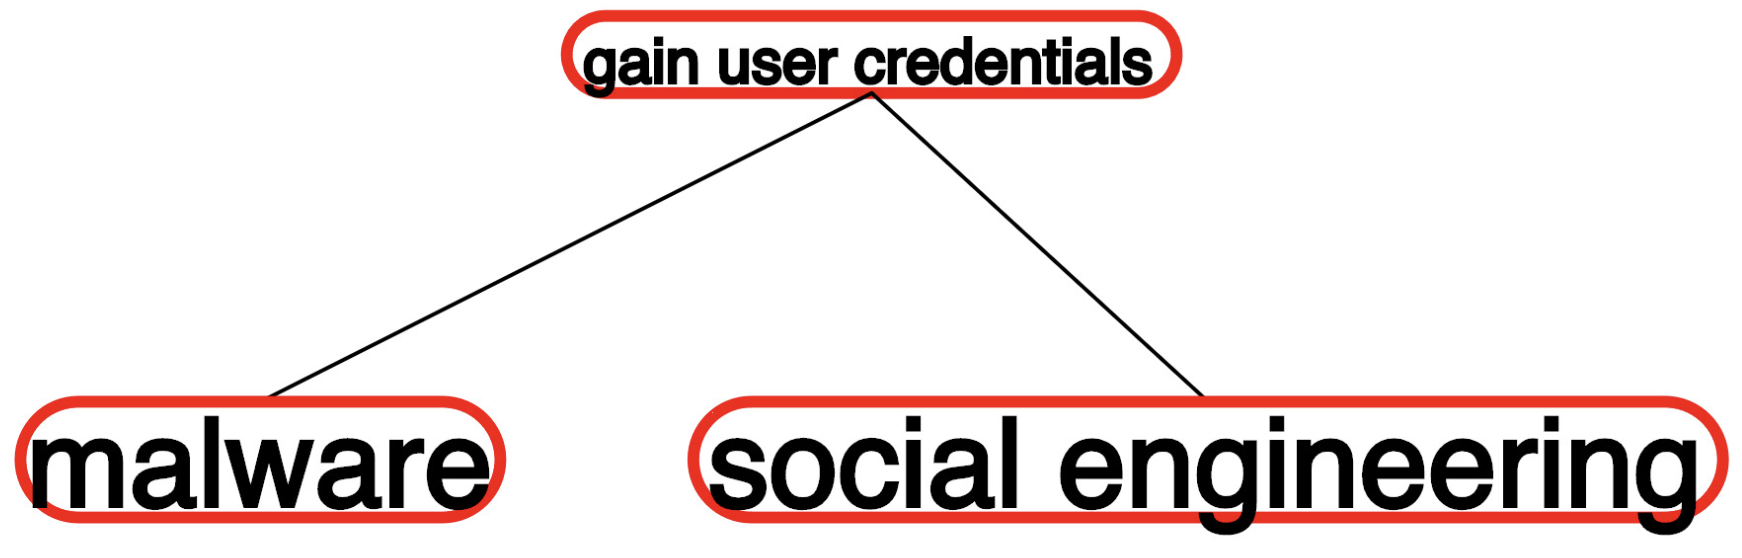
\includegraphics[width=\linewidth]{img/NodeFlip1.png}
    \end{subfigure}
    \begin{subfigure}{.45\linewidth}
        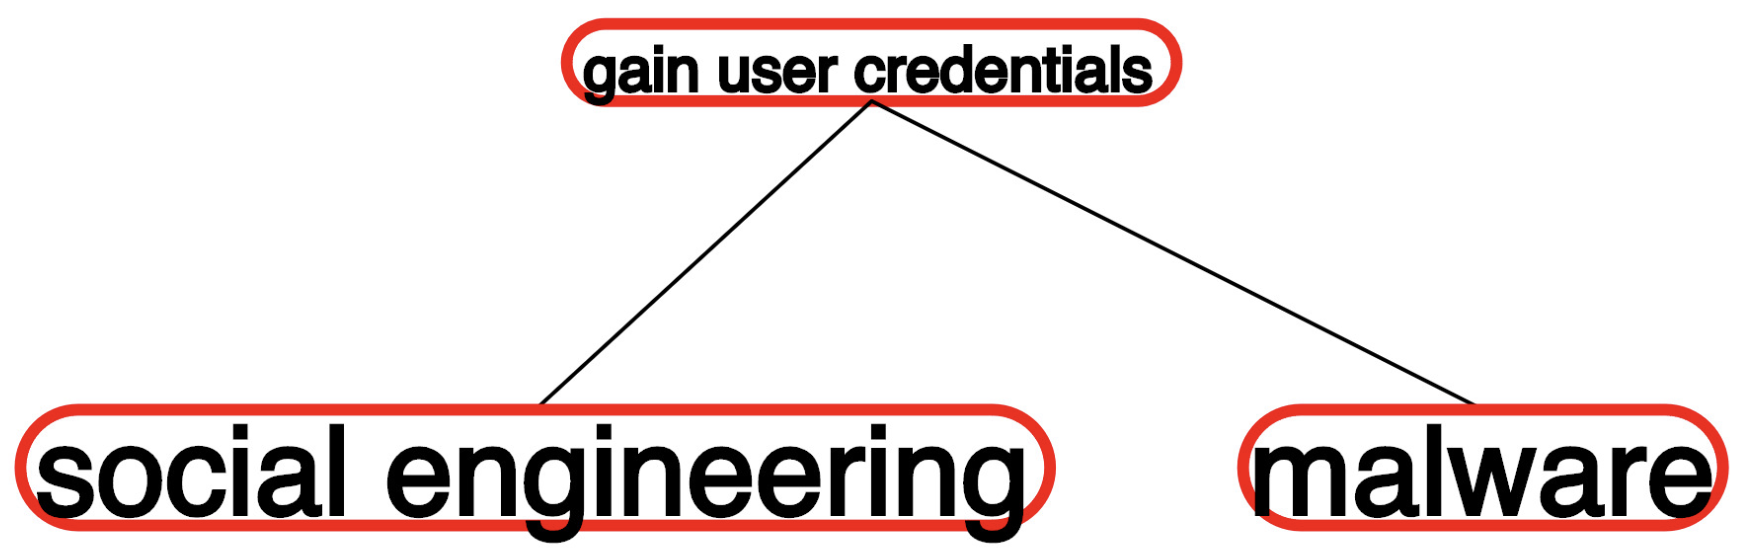
\includegraphics[width=\linewidth]{img/NodeFlip2.png}
    \end{subfigure}
    \caption{Two attack trees (subtrees of the example in Figure~\ref{fig:tartgetAT}) with identical information but different node order. These trees would evaluate to have a distance of 2 (two replacement operations).}
    \label{fig:nodeflipping}
\end{figure}

Attack trees, by virtue of their construction, tend to be organized in levels of abstraction. That is, with each new level of an attack tree, the nodes are given to be more specific than the nodes in the previous level. This is shown in Figure~\ref{fig:tartgetAT}, where the root node is given to be the most abstract (as the overall goal), while the leaf nodes are the most concrete (as the individual actions). From this, we find siblings in an attack tree to be on the same level of abstraction. As such, the order of siblings can be changed without affecting the meaning of the attack tree. By checking the order of sibling sets between the two attack trees




\subsubsection{Semantic mapping}

Zhang and Shasha motivate and validate their approach by creating a node mapping between the two trees (source and target)~\cite{zhang_simple_1989}. How this mapping is created was not a contribution of that work; however, simple rules for defining mappings based on node placement were included. For example, two nodes could only be mapped if they shared the same placement in terms of parents and siblings. A left-most sibling could not be mapped to a right-most sibling, even if they were the same node. This is part of the reasoning applied to establish that creating this mapping, and thus defining optimal tree-edit distance for unordered trees is an MAX SNP-hard problem~\cite{zhangMAXSNPhardResults1994}.

We adapt the idea of a mapping to instead map nodes based on a comparison of semantic label embeddings. Starting with the root nodes of both source and target trees, we create a matrix of all semantic similarities between the children of these nodes. Starting with the two nodes with the highest label semantic similarity, we map those two nodes together and remove the row and column corresponding to that value from the similarities matrix. Finally, we reorder the children in each tree such that mapped nodes have the same left-wise index. We then repeat this process until the similarities matrix is empty. We then repeat this process for all newly added mappings. This process is shown in Algorithm~\ref{alg:sibling_reorder}. It is a top down algorithm, starting from the root node and working down to the leaf nodes.

This methodology is not guaranteed to return smaller edit distance. If it were, this would represent a polynomial approximate solution to an MAX SNP-hard problem. We can construct a counter example by considering two trees with some identical subtree. If prior to the mapping the parent nodes of these subtrees were in the correct order such that these identical subtrees would be matched by the Zhang and Shasha algorithm, and the process of creating the semantic mapping caused the parent nodes of these identical subtrees to be placed out of order, the tree edit distance would increase as a result of our mapping step, as the previous matching operations (which are given to not have a cost) would no longer occur in the Zhang and Shasha algorithm, and would likely be replaced with a large series of add and remove operations (which each incur a cost). However, this scenario is only possible if the root nodes of these identical subtrees are not semantically mapped together, which is highly unlikely to occur in practice. This potential could be mitigated by calculating the tree edit distance twice: once with semantic node remapping and once without, to check that the node mapping has not increased edit distance. Such a step would not increase the computational complexity of the overall calculation, but would ensure that the worse case scenario does not occur.





\begin{algorithm}
    \caption{An algorithm to reorder siblings based on semantic similarity}
    \label{alg:sibling_reorder}
    \begin{algorithmic}
        \State Two attack trees $T_1$ and $T_2$ according to Definition~\ref{def:attack-tree} with $a$ and $b$ total nodes respectively
        \State $M$ is the mapping of nodes between $T_1$ and $T_2$ \Comment{We give $m[0]$ and $m[1]$ to be the source and target nodes of a mapping for $m \in M$}
        \State $M \gets T_1[a]\mapsto T_2[b]$\Comment{Root nodes are always mapped}
        \For{$m \in M$}

        \State $D \gets []$ \Comment{Matrix of semantic similarity values}
        \For{left-wise index $i$ in $m[0].\text{children}$}
        \For{leftwise index $j$ in $m[1].\text{children}$}
        \State $D[i][j] \gets$
        \State$\text{  }\text{  }\text{  }\text{  }\text{  }\text{  }\text{  }\text{  }\text{  }\delta(m[0].\text{children}[i].\text{label}, m[1].\text{children}[j].\text{label})$
        \EndFor
        \EndFor
        \State $M_t \gets \emptyset$ \Comment{Temporary set of mappings}
        \While{$D$ is not empty}
        \State $i, j \gets \text{argmax}(D)$ \Comment{Largest value in $D$}
        \State $M_t \gets M_t \cup m[0].\text{children}[i]\mapsto m[1].\text{children}[j]$
        \State $D \gets D - i$ \Comment{Remove row $i$}
        \State $D \gets D - j$ \Comment{Remove column $j$}
        \EndWhile
        \For{$p$ in $M_t$}
        \If{indicies $i$, $j$ of $p$ are not equal}
        \State{Swap nodes $i$ and $j$ \textbf{in $T_1$}}
        \EndIf
        \EndFor
        \State $M \gets M \cup M_t$
        \EndFor
    \end{algorithmic}
\end{algorithm}


\subsubsection{Ordered Subtrees}

As we have discussed in Subsections~\ref{sec:background}~and~\ref{sec:refinement-awareness}, there are components of attack trees which can be given to be ordered; namely, \SAND\ attack trees~\cite{jhawar_attack_2015}. While these attack trees are out of scope for our definition and contribution, they are a common extension on the attack tree formalism~\cite{lallieReviewAttackGraph2020}. If a \SAND\ node exists within an attack tree, Algorithm~\ref{alg:sibling_reorder} can be modified to check the relationship between children of nodes and to directly map ordered nodes together regardless of label semantic similarity. As stated previously, this is out of scope for our contribution; the validation and testing of such an approach will have to be attended to in a future work.
